\chapter{Propuesta}\label{chapter:proposal}
	La propuesta de solución consiste en varios pasos. Primero se capturan las señales de los sensores y se almacenan.
	Luego, se realiza un preprocesado de los datos, para eliminar datos que sean erróneos. Durante este proceso, también
	se extraen ciertas características importantes a partir de las ya existentes en los datos obtenidos durante la fase
	de captura de señales. Una vez se tengan los datos que se quieren estructurados, se pasa a una fase de detección de
	anomalías utilizando algunos métodos heurísticos y de aprendizaje no-supervisado. Las anomalías que se extraigan con
	este proceso son etiquetadas con un método que utiliza la distancia de la ubicación de las lecturas a ciertas marcas
	previamente etiquetadas a mano. Luego se realiza un proceso de selección de características utilizando varios métodos 
	para determinar las más relevantes a la hora de clasificar las anomalías en bache o no bache. Finalmente, se realiza 
	un proceso de selección de modelos e hiperparámetros, mediante el cual se busca un algoritmo y una configuración de 
	hiperparámetros que maximice el \emph{F1 score}.

\section{Captura de señales}
	Las señales que se consideraron capturar son las proporcionadas por sensores como el \textbf{acelerómetro},
	el \textbf{giroscopio} y el \textbf{GPS}, pues son los sensores más comunes en los teléfonos inteligentes. El
	\textbf{acelerómetro}, como se explica en la literatura, permite medir en tiempo real la aceleración(rapidez de
	cambio de la \textbf{velocidad}) en $m/s^2$ con respecto a los 3 ejes principales, y en el caso de los
	acelerómetros integrados en los teléfonos inteligentes permite medir la aceleración en los 3 ejes
	principales del dispositivo en cuestión. Estos 3 ejes(figura \ref{fig:2}) se encuentran ubicados, si se sostiene el
	dispositivo de la forma usual, de la siguiente manera:

	\begin{itemize}
		\item eje X: Va de un lado del dispositivo a otro (lateral).
		\item eje Y: Va desde la parte inferior hasta la parte superior del dispositivo (longitudinal).
		\item eje Z: Es ortogonal a la pantalla del dispositivo (vertical).
	\end{itemize}
	
	\begin{figure}[htb]
		\centering
		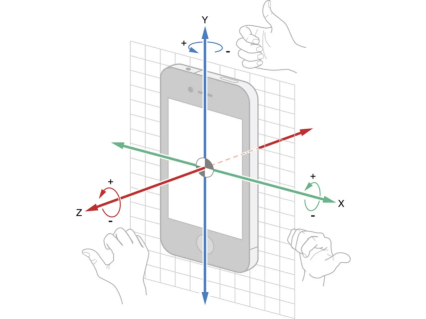
\includegraphics[scale = 0.4]{Graphics/mobile_phone_axis.png}
		\caption{Ejes de un dispositivo móvil}
		\label{fig:2}
	\end{figure}

	Por su parte, los ejes correspondientes a un vehículo(figura \ref{fig:3}) están distribuidos de la siguiente forma:

	\begin{itemize}
		\item eje X: Va de un lado del vehículo a otro (lateral).
		\item eje Y: Va desde la parte trasera hasta la parte delantera del vehículo (longitudinal).
		\item eje Z: Es ortogonal al vehículo, es decir, va desde la parte inferior hasta la parte superior del mismo (vertical).
	\end{itemize}

	\begin{figure}[htb]
		\centering
		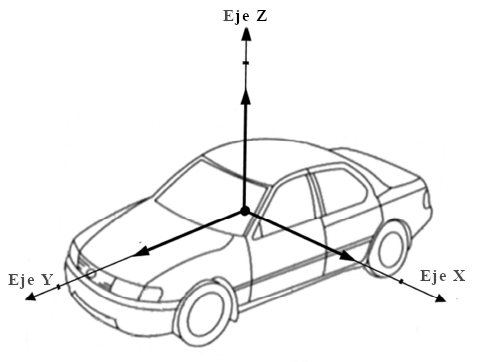
\includegraphics[scale = 0.4]{Graphics/car-axis.jpg}
		\caption{Ejes de un vehículo}
		\label{fig:3}
	\end{figure}

	\subsection{Acelerómetro}
		La señal del \textbf{acelerómetro} mientras el vehículo se desplaza por carreteras en buen estado es bien similar.
		Sin embargo, una vez pasa por encima de un bache ocurre un evento anómalo en el que el vehículo se ve afectado
		por el bache. En ese momento cae brevemente e incluso se inclina momentáneamente hacia un lado (en el caso de un bache
		que afecte una sola rueda). Por esta razón, la señal del \textbf{acelerómetro} en un intervalo de tiempo determinado debe tener
		un comportamiento fuera de lo común que permita identificar el evento en la serie temporal capturada por este sensor.\\
		\indent Tal como se plantea en la literatura, la característica fundamental de un bache son lecturas anormales en el eje
		Z del \textbf{acelerómetro} durante un intervalo de tiempo determinado. También, dicho sensor debe registrar lecturas
		anormales en el eje X si el bache afecta un solo lado del vehículo, pues en este caso el vehículo se inclina violentamente
		hacia un lado por un momento(figura \ref{fig:4}).\\

	\begin{figure}[htb]
		\centering
		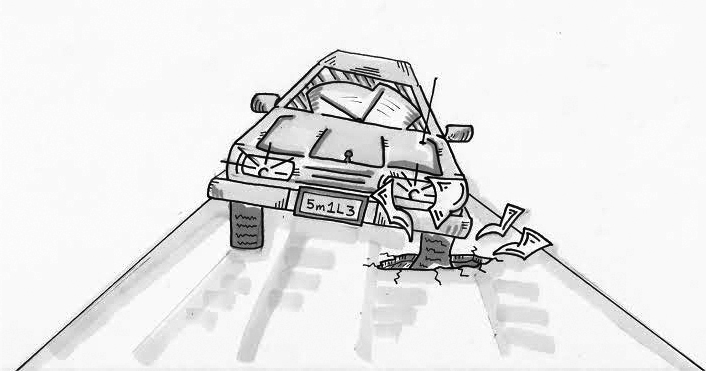
\includegraphics[scale = 0.5]{Graphics/one_side_pothole_vehicle.jpg}
		\caption{Vehículo impactado por un bache en un solo lado}
		\label{fig:4}
	\end{figure}

	\subsection{Giroscopio}
		El \textbf{giroscopio} es otro de los sensores que se considera que aportaría información útil, ya que este sensor 
		mide en $rad/s$ la velocidad angular del dispositivo móvil con respecto a los 3 ejes mencionados previamente. 
		En el momento que un vehículo interactúa con un bache ocurren vibraciones que hacen que el vehículo gire, lo que
		debería generar picos en las lecturas del \textbf{giroscopio} en un intervalo de tiempo. El problema con este sensor es 
		que, a pesar de ser de los más comunes, no es abundante en teléfonos inteligentes de gama baja, por lo que 
		su uso en la propuesta de solución se tiene pensado como algo que permita mejorarla y no algo de lo que esta
		dependa.\\

	\subsection{GPS}
		El \textbf{GPS}(\emph{Global Positioning System}) es el sensor que le permite al dispositivo móvil ubicarse sobre la
		superficie de la tierra utilizando coordenadas de latitud-longitud. Debido a que este sistema utiliza señales para
		comunicarse con satélites en tiempo real, existe una latencia debido al tiempo que le toma a la señal viajar hacia el
		satélite y de vuelta al dispositivo. Además, las condiciones atmosféricas pueden afectar esta latencia, así como el hecho
		de que la señal puede ser reflejada por el terreno, edificios, etc., como por ejemplo, cuando se viaja a través de un
		túnel subterráneo donde la señal no puede llegar.\\
		\indent También es importante destacar que las lecturas que genera el \textbf {GPS} tienen cierto margen de error que varía
		de un dispositivo a otro y que depende de la potencia del sensor en sí. En general, según la literatura, la mediana del error
		en estos sensores es de 5m aproximadamente\brackcite{eriksson2008pothole}, ambos aspectos son importantes a tener en cuenta
		al hacer uso de este sensor. El mismo se puede utilizar para estimar la \textbf{velocidad} a la que viaja el vehículo, lo que
		es necesario, ya que la \textbf{velocidad} es un factor que influye de forma directa en la forma que un vehículo es afectado por
		un bache. Además, con este sensor es posible ubicar en un mapa, aproximadamente, los lugares donde existen baches u otro tipo
		de anomalías, incluso puede ser útil para marcar rutas de viaje y así facilitar algunos aspectos de la propuesta de solución.

	\subsection{Velocidad y frecuencia de muestreo}
		Debido a que la \textbf{velocidad} de un vehículo durante un recorrido no suele ser constante, es necesario que la \textbf
		{frecuencia de muestreo} del \textbf{acelerómetro} y el \textbf{giroscopio} cambie en función de la \textbf{velocidad}
		a la que vaya el vehículo. Pues si el vehículo se desplaza más rápido, será necesario muestrear más para mantener la
		precisión y consistencia de los datos que se generen.\\
		\indent La frecuencia de muestreo se tomó de tal forma que se tuviera una lectura de \textbf{acelerómetro} y \textbf
		{giroscopio} por cada metro. Si el vehículo se desplaza a una \textbf{velocidad} $v$ en $m/s$ y se quiere obtener
		$x$ muestras por cada metro, quiere decir que se necesitan obtener $v * x$ muestras, por lo que la frecuencia de muestreo
		necesaria sería de $v * x Hz$. Como se quiere una sola muestra por cada metro la frecuencia de muestreo
		en este caso particular es de $v Hz$. La actualización de la \textbf{frecuencia de muestreo} ocurre cada vez que se recomputa
		la velocidad, lo que se propuso realizar cada 5 segundos debido a la posible latencia inherente del \textbf{GPS} a la hora
		obtener las lecturas.\\
		\indent Para actualizar de forma correcta la \textbf{frecuencia de muestreo} es necesario conocer la \textbf{velocidad}
		a la que viaja el vehículo, o al menos realizar una estimación aceptable de la misma utilizando los sensores de
		los que dispone el dispositivo móvil. Esta estimación se realizó utilizando las lecturas del \textbf{GPS} y se 
		asignaron frecuencias de muestreo teniendo en cuenta los límites de velocidad existentes en la zona urbana donde 
		se llevaron a cabo los experimentos. Debido a que en Cuba existen muy pocas carreteras donde se permita a
		los vehículos desplazarse a más de 100 km/h y también debido a que la mayoría de los vehículos que circulan en
		el país no alcanzan dicha \textbf{velocidad}, se asumió que esta es la máxima a la que podría desplazarse un
		vehículo a la hora de decidir las frecuencias de muestreo de los sensores.\\
		\indent La frecuencia de muestreo del \textbf{GPS} se fijó constante en 1Hz debido a que es necesario tener 
		la ubicación en tiempo real del dispositivo y buena precisión en las lecturas del propio \textbf{GPS}. Además, 
		muestrear más de una vez por segundo no es necesario, pues la distancia entre una lectura y otra no es considerable.\\

	\subsection{Posición del móvil en el vehículo}
		La posición en la que se coloca el dispositivo móvil en el vehículo a la hora de capturar las señales de los sensores es
		relevante. Esto se debe a que es necesario que las lecturas que se obtengan durante el muestreo sean relevantes y representen
		las características de la carretera por la que viaja el vehículo. Para esto, es necesario colocar el dispositivo móvil de tal 
		forma que la dirección del eje Y del vehículo coincida con la del eje Y del móvil, para que las señales que se capturen
		se correspondan con la realidad. De lo contrario, se deberían realizar ciertos ajustes utilizando algún método de
		transformación de coordenadas para poder obtener lecturas acertadas, sin importar la posición en la que se coloque
		el dispositivo.

\section{Preprocesamiento de los datos}
	Luego de recolectar los datos, se lleva a cabo un preprocesamiento de los mismos para eliminar o corregir ciertos aspectos.
	El primer aspecto de este preprocesamiento es eliminar lecturas donde la precisión del \textbf{GPS} sea mayor que 10 m
	con el objetivo de tener la mayor precisión posible en los datos recopilados.\\
	\indent También, debido a que la frecuencia de muestreo del \textbf{acelerómetro} y el \textbf{giroscopio} es mayor que la del
	\textbf{GPS}, existen varias lecturas consecutivas con un mismo valor de latitud-longitud en ese intervalo de tiempo. Para
	corregir esto se estimaron los valores de latitud-longitud de dichas lecturas utilizando interpolación lineal entre dos lecturas
	de \textbf{GPS} consecutivas.

	\subsection{Extracción de características}
		Durante este proceso, además de corregir y eliminar ciertos datos, también se extrajeron características. Entre ellas,
		algunas estadísticas.  Luego se incorporaron a cada uno de los datos. Estas características se extrajeron con el objetivo
		de tener un juego de datos que brindara más información acerca de la naturaleza del problema, y así, tentativamente,
		mejorar la calidad de la propuesta.\\

		Las características no estadísticas extraídas fueron:\\

		\begin{itemize}
			\item X/Z: Cociente entre la aceleración en el eje X y la aceleración en el eje Z.
			\item MaxZRatio: Cociente entre la aceleración en el eje Z y el máximo valor de aceleración en el eje Z.
			\item MinZRatio: Cociente entre la aceleración en el eje Z y el mínimo valor de aceleración en el eje Z
			\item SpeedVsZ: Cociente entre la velocidad y la aceleración en el eje Z.
		\end{itemize}

		Las características estadísticas extraídas fueron:\\

		\begin{itemize}
			\item MeanDevAccelX: Desviación del valor de la aceleración en el eje X con respecto a la media.
			\item MedianDevAccelX: Desviación del valor de la aceleración en el eje X con respecto a la mediana.
			\item MeanDevAccelY: Desviación del de la aceleración en el eje Y con respecto a la media.
			\item MedianDevAccelY: Desviación del valor de la aceleración en el eje Y con respecto a la mediana.
			\item MeanDevAccelZ: Desviación del valor de la aceleración en el eje Z con respecto a la media.
			\item MedianDevAccelZ: Desviación del valor de la aceleración en el eje Z con respecto a la mediana.
			\item MeanDevGyroX: Desviación del valor del giroscopio en el eje X con respecto a la media.
			\item MedianDevGyroX: Desviación del valor del giroscopio en el eje X con respecto a la mediana.
			\item MeanDevGyroY: Desviación del valor del giroscopio en el eje Y con respecto a la media.
			\item MedianDevGyroY: Desviación del valor del giroscopio en el eje Y con respecto a la mediana.
			\item MeanDevGyroZ: Desviación del valor del giroscopio en el eje Z con respecto a la media.
			\item MedianDevGyroZ: Desviación del valor del giroscopio en el eje Z con respecto a la mediana.
		\end{itemize}

\section{Detección de anomalías}
	Los baches no son más que anomalías en la carretera. Teniendo en cuenta esto, se propuso detectar dichas anomalías utilizando
	2 enfoques. Primero, intentar identificar las anomalías utilizando los métodos heurísticos sugeridos en la literatura basados
	en umbrales. Segundo, emplear algoritmos de aprendizaje de máquinas para detectar anomalías.\\
	\indent Los métodos heurísticos que se utilizaron en la propuesta fueron \textbf{Z-THRESH}, \textbf{Z-DIFF} y \textbf{G-ZERO}.
	Estos solo hacen uso de las lecturas del \textbf{acelerómetro} para determinar la existencia de una anomalía. Por otro lado, los
	métodos de aprendizaje de máquinas que se probaron fueron \textbf{DBSCAN}, \textbf{OPTICS} y \textbf{One Class SVM} utilizando 
	6 características, las lecturas de los 3 ejes del \textbf{acelerómetro}, y además las lecturas de los 3 ejes del \textbf{giroscopio}.
	Este último sensor se incluyó, pues se consideró que sus lecturas pueden ser significativas a la hora de determinar la existencia de una 
	anomalía. Este proceso de detección de anomalías se aplicó a cada una de las series temporales obtenidas como resultado del muestreo
	de los sensores del dispositivo móvil.

\section{Etiquetado de anomalías}
	Luego de haber detectado las anomalías, es necesario llevar a cabo un proceso de etiquetado para poder utilizar los datos en la siguiente
	fase de la propuesta. Para esto se utilizaron las anomalías extraídas de la serie temporal y una lista de marcas. Estas marcas se realizaron
	manualmente a lo largo de la misma ruta con la cual se generaron las series temporales e indican la presencia de un bache en cierta
	ubicación, con coordenadas de latitud-longitud.\\
	\indent Para asignar la etiqueta de bache a una anomalía se busca en un radio predefinido si existe una marca de bache, de lo contrario, se le
	asigna la etiqueta de no bache. Debido a que es imposible determinar exactamente el punto donde el vehículo hizo contacto con el bache
	utilizando el \textbf{GPS}, a causa del error inherente del sensor, este proceso de etiquetado tiene cierto error. Este error puede ocasionar
	que anomalías que no sean baches sean etiquetadas como tal debido a que exista una marca que indique la presencia de un bache en un radio
	cercano a esta.

\section{Selección de características}
	Ya con los datos etiquetados, lo próximo que se propuso fue llevar a cabo un proceso de selección de características utilizando métodos como
	\emph{Forward Selection}, \emph{Backward Selection} y \emph{Recursive Feedback Elimination}. De esta forma, se podrían determinar cuáles de las 
	características que posee nuestro juego de datos son mejores para predecir si una anomalía es bache o no bache. Con lo cual se podría determinar
	automáticamente la existencia de un bache en la carretera.

\section{Selección de modelo}
	Una vez se sabe qué características son las mejores para predecir si una anomalía es bache o no, se llevó a cabo un proceso de selección de
	modelo. La métrica de evaluación que se escogió fue el \emph{F1 score} porque se consideró que un equilibrio entre \emph{precision} y
	\emph{recall} es más relevante que el \emph{accuracy} para el problema en cuestión. Este proceso de selección de modelo tiene el
	objetivo de determinar entre varios modelos definidos cuál obtiene mejor rendimiento con respecto a la métrica seleccionada utilizando los datos
	del problema. Los modelos entre los cuales se propuso escoger son: \textbf{KNN}, árboles de decisión, \emph{Random Forest}, regresión logística y
	\textbf{SVM}.\\
	\indent Junto con este proceso de selección de modelo también se llevó a cabo una selección de hiperparámetros que permita determinar con
	cuáles de estos el modelo arroja mejores resultados. Finalmente, se evaluó el rendimiento del modelo analizando el comportamiento de la métrica
	de evaluación en un conjunto de prueba.
